\begin{figure*}[!t]
\centering
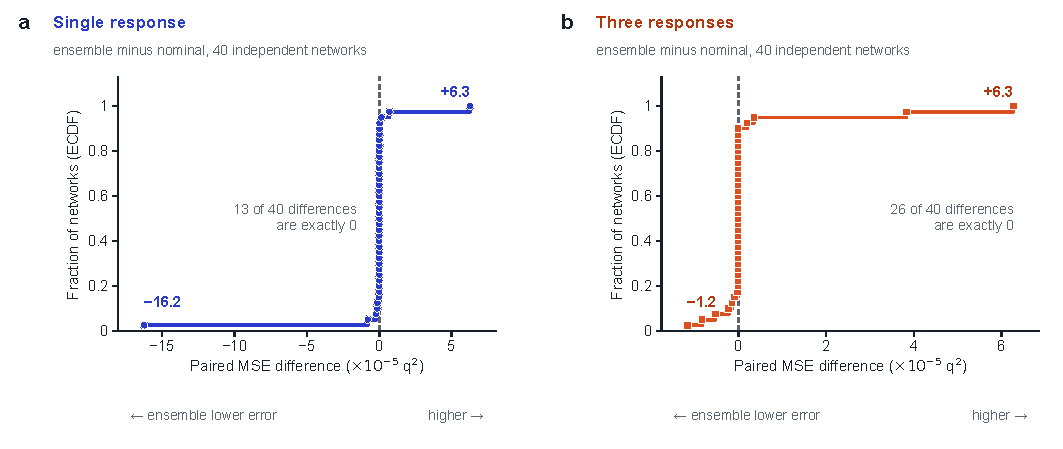
\includegraphics[width=\textwidth]{../../03_figures/supplementary_v4/figS1_complete_paired_distributions_v4.pdf}
\setcounter{figure}{0}
\caption{\textbf{Complete paired primary differences.} Each panel shows all 40
independent network-level ensemble-minus-nominal raw-MSE differences for
the single-response (a) and three-response (b) comparison, including
exact ties and the influential networks; the step curve is the empirical
distribution function and every sorted value is drawn as a marker. The
horizontal axis is in units of 10\textsuperscript{−5}
q\textsuperscript{2}; negative values favour the ensemble. Extreme
values (−16.2 and +6.3 in a; −1.2 and +6.3 in b) are labelled, not
truncated. Exactly 13 (a) and 26 (b) of the 40 differences are zero. The
distributions are descriptive; no interval is drawn, and the primary
intervals remain those in Table 1 and Fig. 3. No equivalence margin was
specified, and nothing here shows that the two selection rules perform
alike.}
\label{sfig:1}
\end{figure*}

\begin{figure*}[!t]
\centering
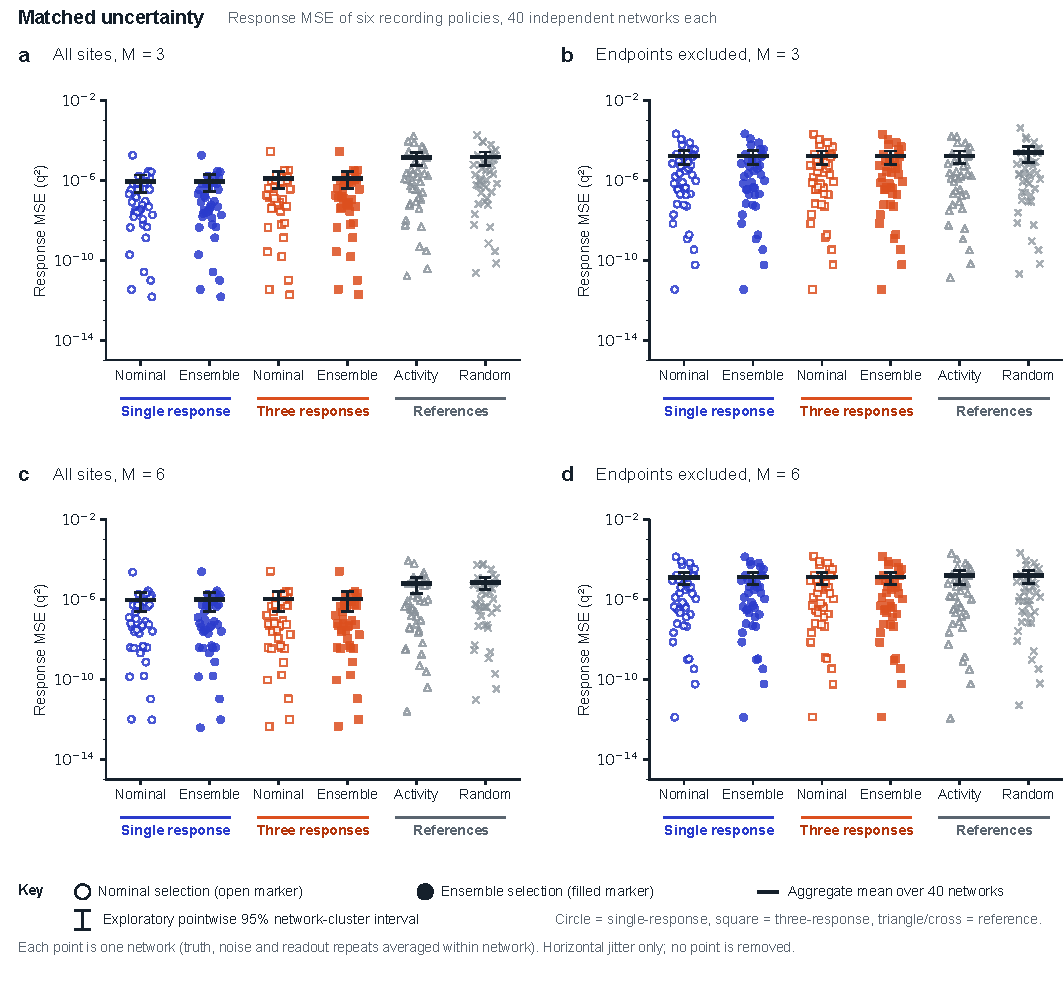
\includegraphics[width=\textwidth]{../../03_figures/supplementary_v4/figS2_matched_conditions_v4.pdf}
\setcounter{figure}{1}
\caption{\textbf{All recording conditions under matched uncertainty.} Panels a--d
show all-site/M = 3, endpoint-excluded/M = 3, all-site/M = 6 and
endpoint-excluded/M = 6. For each of six policies (nominal and ensemble
single-response, nominal and ensemble three-response, activity, random)
every one of the 40 independent networks is shown as one point, with
truth, noise and readout repeats averaged within network. Thick black
bars are the aggregate means and thin black lines the exploratory
pointwise 95\% network-cluster intervals from the frozen summary table.
Open markers denote nominal and filled markers ensemble selection;
horizontal jitter only separates overlapping points. All panels share
the logarithmic response-MSE axis (10\textsuperscript{−15} to
10\textsuperscript{−2}). No point or tail is removed. Intervals are not
multiplicity-adjusted and no pairwise or equivalence claim is made.}
\label{sfig:2}
\end{figure*}

\begin{figure*}[!t]
\centering
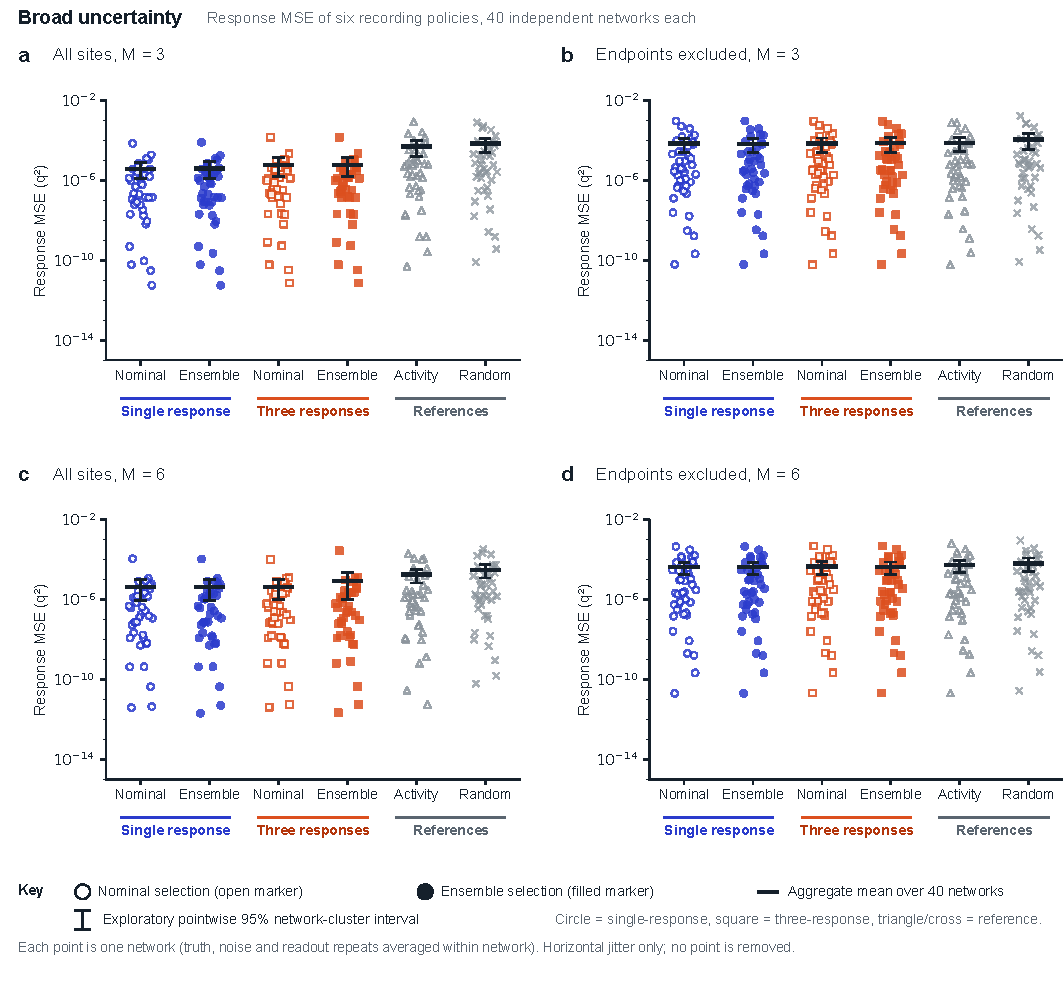
\includegraphics[width=\textwidth]{../../03_figures/supplementary_v4/figS3_broad_conditions_v4.pdf}
\setcounter{figure}{2}
\caption{\textbf{All recording conditions under broad uncertainty.} As
Supplementary Fig. 2 for the broad prior: panels a--d show all-site/M =
3, endpoint-excluded/M = 3, all-site/M = 6 and endpoint-excluded/M = 6;
40 independent networks per policy and panel; black bars and lines are
aggregate means and exploratory pointwise 95\% network-cluster
intervals; shared logarithmic axes; open nominal, filled ensemble;
jitter is horizontal only. The primary comparison in Fig. 3 corresponds
to panel b. No method-specific tail is removed, and the panels do not
support any claim of equivalence or superiority.}
\label{sfig:3}
\end{figure*}

\begin{figure*}[!t]
\centering
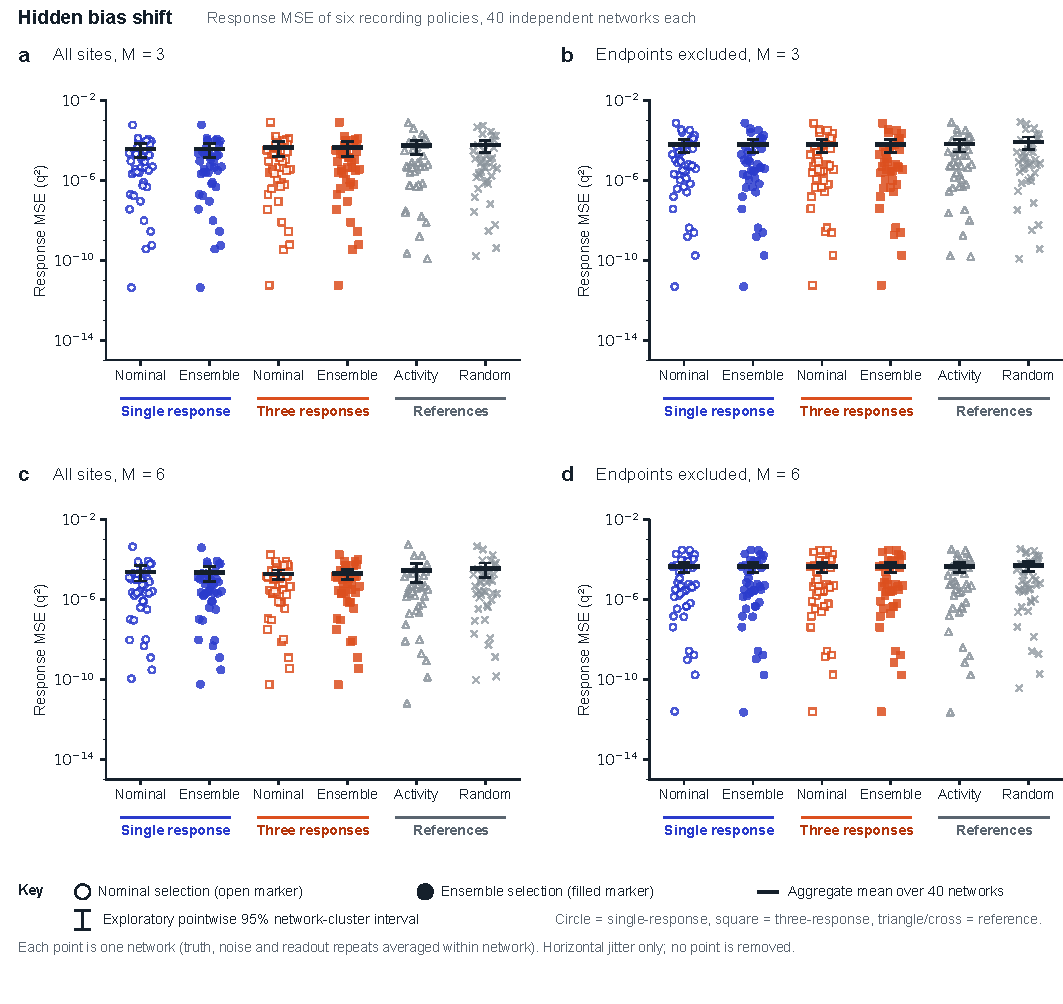
\includegraphics[width=\textwidth]{../../03_figures/supplementary_v4/figS4_bias_shift_conditions_v4.pdf}
\setcounter{figure}{3}
\caption{\textbf{All recording conditions under hidden bias shift.} As
Supplementary Fig. 2 for the hidden-bias-shift condition: panels a--d
show all-site/M = 3, endpoint-excluded/M = 3, all-site/M = 6 and
endpoint-excluded/M = 6; 40 independent networks per policy and panel;
black bars and lines are aggregate means and exploratory pointwise 95\%
network-cluster intervals; shared logarithmic axes; open nominal, filled
ensemble; jitter is horizontal only. No data are filtered, and the
intervals are descriptive and not multiplicity-adjusted.}
\label{sfig:4}
\end{figure*}

\begin{figure*}[!t]
\centering
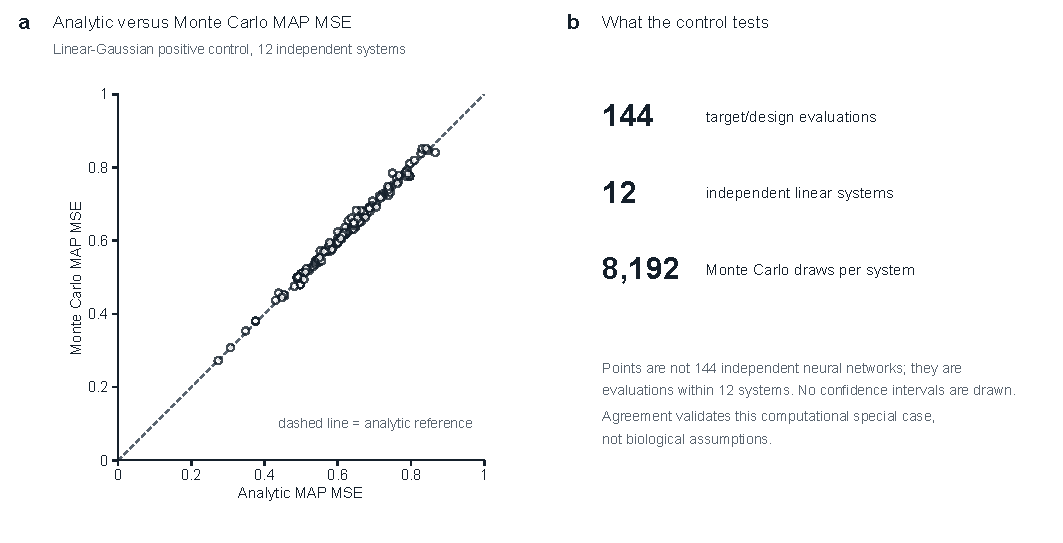
\includegraphics[width=\textwidth]{../../03_figures/supplementary_v4/figS5_linear_positive_control_v4.pdf}
\setcounter{figure}{4}
\caption{\textbf{Nondegenerate linear-Gaussian positive control.} All 144
target/design evaluations from 12 independent linear systems compare the
analytic MAP MSE (horizontal) with the Monte Carlo MSE from 8,192 draws
per system (vertical); the dashed identity line is the analytic
reference. The independent unit is the system (n = 12); the 144 points
are evaluations within systems, not independent neural networks, and no
confidence intervals are displayed. Agreement validates this
computational special case only; it does not validate biological
assumptions.}
\label{sfig:5}
\end{figure*}
